\documentclass{beamer}

\usepackage{fontspec}
\usepackage{xeCJK}
\setCJKmainfont[BoldFont=Noto Serif CJK TC Bold]{Noto Serif CJK TC}
\XeTeXlinebreaklocale "zh"
\XeTeXlinebreakskip = 0pt plus 1pt
\linespread{1.3}
\allowdisplaybreaks

\usepackage{color}
\usepackage{booktabs}
\usepackage{tabularx}
\usepackage{caption}
\usepackage{tikz}
\usepackage{verbatim}
\usepackage{pgfplotstable}
\pgfplotsset{width=12cm}
\pgfplotsset{height=7cm}
\pgfplotsset{compat=1.13}

\usetheme{EastLansing}
\usetikzlibrary{positioning}
\useinnertheme{rectangles}
\usefonttheme{professionalfonts}

\newcommand{\lw}{0.8mm}
\setbeamercovered{transparent}


%\AtBeginSection[]
%{
  %\begin{frame}<beamer>
	%\frametitle{報告大綱}
	%%\frametitle{RoadMap}
    %\tableofcontents[currentsection]
  %\end{frame}
%}

\title{Progress Report}
\subtitle{\textcolor[rgb]{0.00,0.50,1.00}{{Speech Processing \& Machine Learning Laboratory}}}
\author{徐瑞陽}
\date{2019/09/25}
\begin{document}

\begin{frame}
\maketitle
\end{frame}



\begin{frame}
\frametitle{Outline}
\tableofcontents
\end{frame}

\section{Background}
\begin{frame}[t]{Introduction}
  \begin{center}
    Apply meta learning to speech processing 
  \end{center}

  \pause

  Existing application on \textbf{Speaker Adaptative Training} (SAT)
  \begin{itemize}
    \item Meta-SGD (Interspeech 2018)
    \item MAML (ASRU 2019 ?)
  \end{itemize}

  The above 2 use TDNN model to do classification on phoneme level
\end{frame}

\begin{frame}[t]{Introduction}
  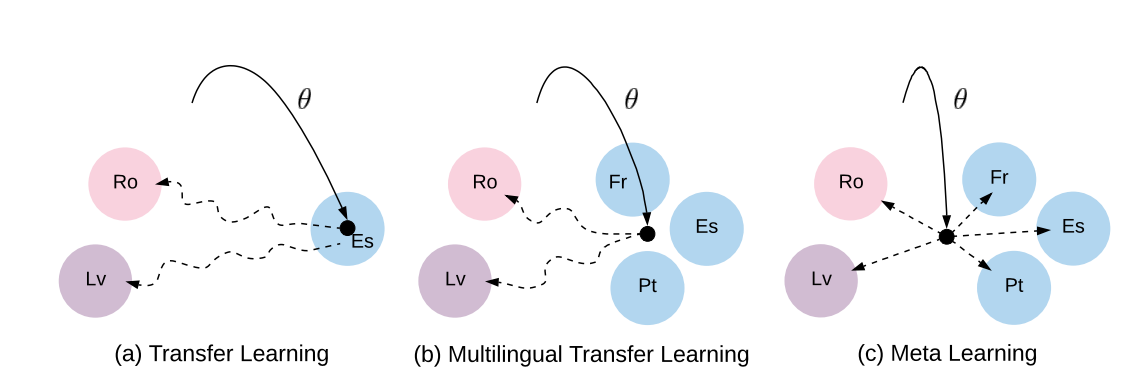
\includegraphics[width=0.9\textwidth]{fig/Meta-motivation.png}

  Our setting
  \begin{itemize}
    \item Language Adaptative Training
    \item End-to-end ASR: more realistic in low-resource regime
    \item Pluggable: no need to have target corpus during pretraining
  \end{itemize}
\end{frame}

\begin{frame}[t]{Implementation}
  \begin{itemize}
    \item Corpus: IARPA-BABEL (17 languages)
    \item Model structure: LAS
    \item Meta-learner: \textbf{Reptile}, FOMAML, Leap
  \end{itemize}
  \center 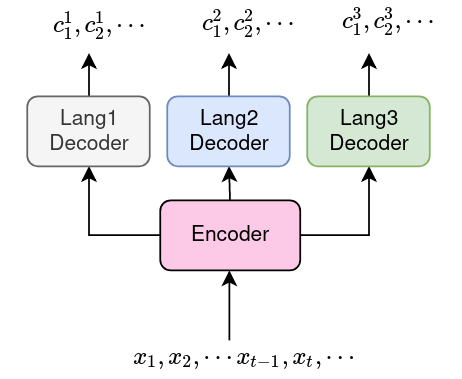
\includegraphics[width=0.5\textwidth]{fig/MultiTaskASR.png}
\end{frame}

\begin{frame}{Proposed method}
  Meta-learn
  \begin{itemize}
    \item Whole encoder
    \item Last layer of encoder (pretrain using multitask learning, then freeze till penultimate layers of encoder)
  \end{itemize}
  \pause
  \center 都失敗惹 QQ
\end{frame}

\section{Pretraining language selection}

%\section{Meta-Learning With Latent Embedding Optimization}
%\begin{frame}
  %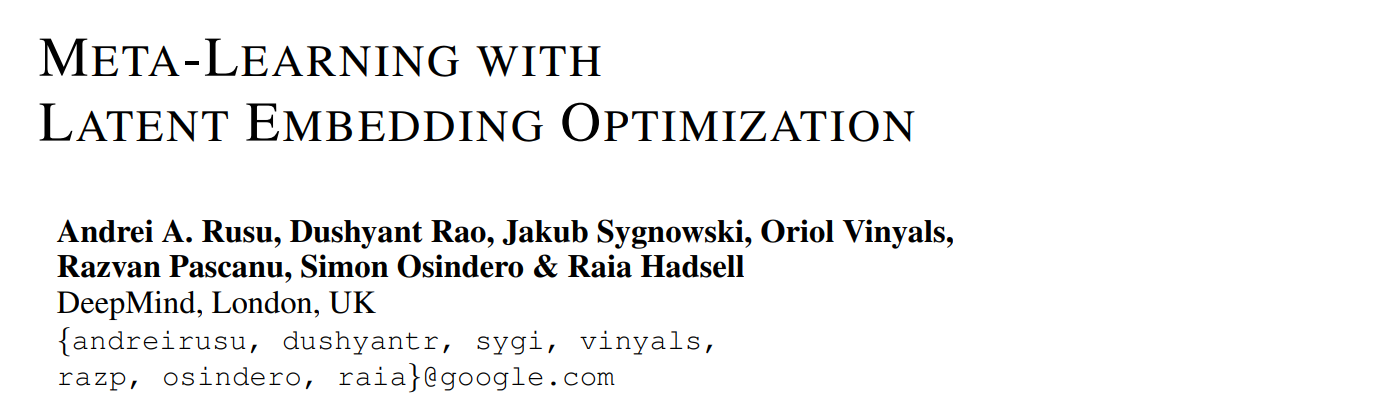
\includegraphics[width=\textwidth]{fig/LEO.png}
  %\center ICLR 2019
%\end{frame}



%\section{MISC}
\begin{frame}
	\begin{center}
    %\weib{\LARGE{謝謝聆聽!}}
    \LARGE{Questions?}
	\end{center}
\end{frame}

\end{document} 
